\documentclass[10pt]{article}
\usepackage[a4paper,margin=2.2cm]{geometry}
\usepackage[T1]{fontenc}
\usepackage{lmodern,microtype}
\usepackage{amsmath,amssymb,amsfonts,bm}
\usepackage{graphicx,booktabs,multirow,xcolor,longtable}
\usepackage[hidelinks]{hyperref}
\usepackage{url}
\usepackage[numbers,sort&compress]{natbib}
\usepackage{caption}
\captionsetup{font=small,labelfont=bf}
\newcommand{\caramel}{\texttt{caramel}}
\newcommand{\josie}{JOSIE}
\newcommand{\pending}{\textcolor{gray}{\textit{pending}}}
\newcommand{\fig}[3][\linewidth]{\begin{figure}[t]\centering\includegraphics[width=#1]{figures/#2.pdf}\caption{#3}\label{fig:#2}\end{figure}}

\title{\caramel{}: A Text-Free Full-Duplex Speech Model\\[2pt]
\large Architecture, Pre-training, Inference, and Post-training into a Voice Assistant}
\author{G\"okdeniz G\"ulmez}
\date{November 2026 \\ \small Technical report. Pre-training results are those of the \texttt{caramel-1} release~\cite{caramel1}; post-training is new in this report.}

\begin{document}
\maketitle

\begin{abstract}
We describe \caramel{}, a 413.2M-parameter speech-to-speech model that learns conversation from audio alone. It has never seen text, and it contains no voice-activity detector and no turn-taking rule: every 80\,ms it reads the Mimi codec tokens of both speakers and writes the next eight tokens of its own voice, so \emph{when} to speak is predicted exactly like \emph{what} it sounds like.
The model factorises each frame over time with a 16-layer temporal transformer and over codebooks with a 6-layer depformer, with the acoustic codebooks delayed by one frame.
\texttt{caramel-1} was pre-trained on 11{,}555 hours of public speech (5{,}743\,h two-speaker, 5{,}812\,h one-speaker; 6.2B unique tokens, about 33B seen) that was selected with a 13-statistic \emph{closeness score}, in three stages taking about 2\,h\,15\,min on H100s.
Two copies of the model hold real-time conversations with each other, with overlap (8.8\% vs.\ 9.0\%), silence and words-per-minute close to real people; it runs about $11\times$ real time on a GPU and about $4\times$ for both copies on an M3 Pro laptop.
We then post-train \caramel{} into a voice assistant, \josie{}, using 1{,}431 synthetic full-duplex conversations (151.3\,h) with barge-ins, holds and backchannels. A both-sides fine-tune lowers dev loss from 1.636 to 1.321 but learns to interrupt and to speak in user voices; we analyse this failure, introduce a single-side objective, a two-stage synthetic recipe and a GRPO/DPO stage with event-based duplex rewards. Every number is taken from the repository and its logs; results that do not exist yet are marked as pending.
\end{abstract}

\tableofcontents
\newpage

%=====================================================================
\section{Introduction}
Human conversation is full-duplex. People overlap, backchannel (``mm-hm''), start a turn before the last one ends, and negotiate interruptions within a fraction of a second. Cascaded assistants (ASR $\to$ LLM $\to$ TTS) impose a half-duplex structure from outside, typically with a voice-activity detector and an end-of-turn rule. Full-duplex spoken language models such as dGSLM~\cite{nguyen2023dgslm} and Moshi~\cite{defossez2024moshi} instead model both speakers' audio jointly, so turn-taking emerges from data.

\caramel{} is a deliberately minimal member of this family. It has no text pathway (unlike Moshi's inner monologue), no explicit turn model, and no special conversational machinery; its human-like timing comes from the data selection and the training setup. The design hypothesis, borrowed from the bitter lesson, is that more and better-matched conversational audio is what matters.

This report covers the whole model (Fig.~\ref{fig:fig10_lifecycle}):
\begin{itemize}\itemsep0pt
\item \textbf{Architecture} (\S\ref{sec:arch}): codec, token layout and delays, the temporal transformer and depformer, embeddings, heads and loss, with a parameter count derived from the configuration.
\item \textbf{Pre-training data} (\S\ref{sec:data}): the closeness score, sourcing, speaker separation and tokenisation.
\item \textbf{Pre-training recipe} (\S\ref{sec:pretrain}): three stages, schedule, batching, speaker-swap augmentation, evaluation and correctness checks.
\item \textbf{Inference} (\S\ref{sec:infer}): streaming with KV caches, self-play, the live duplex loop and speed.
\item \textbf{Evaluation of \texttt{caramel-1}} (\S\ref{sec:eval}).
\item \textbf{Post-training into \josie{}} (\S\ref{sec:post}): synthetic data, objectives, experiments and an RL stage.
\end{itemize}

\fig{fig10_lifecycle}{The \caramel{} lifecycle covered by this report. Everything up to \texttt{caramel-1} is the released pre-training~\cite{caramel1}; the purple and red boxes are post-training introduced here (status in brackets).}

%=====================================================================
\section{Related work}
\paragraph{Textless spoken language modelling.} GSLM~\cite{lakhotia2021gslm} and AudioLM~\cite{borsos2023audiolm} showed that language models over discrete speech units learn lexical and prosodic structure without text. Neural codecs such as SoundStream~\cite{zeghidour2021soundstream} and EnCodec~\cite{defossez2022encodec} supply residual multi-codebook tokens; MusicGen~\cite{copet2023musicgen} popularised codebook delay patterns for parallel prediction.
\paragraph{Full-duplex dialogue.} dGSLM~\cite{nguyen2023dgslm} modelled two unit streams with a two-tower transformer trained on Fisher telephone conversations and produced realistic overlaps and backchannels. Moshi~\cite{defossez2024moshi} introduced the Mimi codec, the temporal-transformer/depformer factorisation that \caramel{} adopts, and a text inner monologue; it also used synthetic multi-stream dialogues for instruction tuning. SyncLLM~\cite{veluri2024syncllm} synchronises an LLM with a real-time clock for full-duplex dialogue. Seamless Interaction~\cite{agrawal2025seamless} provides about 4{,}000\,h of dyadic recordings with one track per participant.
\paragraph{Speech assistants on LLMs.} SpeechGPT~\cite{zhang2023speechgpt}, Mini-Omni~\cite{xie2024miniomni} and LLaMA-Omni~\cite{fang2024llamaomni} add speech input/output to a text LLM; their dialogue remains turn-based. \caramel{} has no text pathway, so assistant behaviour must be transferred \emph{through audio}.
\paragraph{Training components.} We use RoPE~\cite{su2021roformer}, SwiGLU~\cite{shazeer2020glu}, RMSNorm~\cite{zhang2019rmsnorm} in a Transformer~\cite{vaswani2017attention}, AdamW~\cite{loshchilov2019adamw} with a cosine schedule~\cite{loshchilov2017sgdr}, and for RL GRPO~\cite{shao2024deepseekmath} with PPO clipping~\cite{schulman2017ppo} or DPO~\cite{rafailov2023dpo}. Evaluation uses UTMOS~\cite{saeki2022utmos} and ECAPA-TDNN~\cite{desplanques2020ecapa}. The timing target is Dessa~\cite{dessa}.

%=====================================================================
\section{Architecture}
\label{sec:arch}

\subsection{Audio codec and token layout}
\caramel{} never touches waveforms. Mimi (the codec of Moshi; weights from \texttt{kyutai/moshiko-pytorch-bf16}) maps 24\,kHz audio to $12.5$ frames per second, i.e.\ one frame per $1920$ samples ($80$\,ms). Of Mimi's residual codebooks only the first $K=8$ are kept, each with $V=2048$ entries. Codebook 0 is the semantic codebook and carries mostly what is said; codebooks 1--7 carry voice and room. The token rate of one speaker is therefore
\begin{equation}
r = 12.5\ \tfrac{\text{frames}}{\text{s}}\times 8\ \tfrac{\text{tokens}}{\text{frame}} = 100\ \tfrac{\text{tokens}}{\text{s}},\qquad 3600\,r = 360{,}000\ \text{tokens per hour}.
\end{equation}
A conversation is a matrix $\mathbf{x}\in\{0,\dots,V{-}1\}^{T\times 16}$: columns 0--7 are the speaker being modelled (``me'', A) and columns 8--15 the other speaker (B) (Fig.~\ref{fig:fig2_tokens}). One-speaker clips have width 8; the missing speaker is filled with $-1$.

\fig[.92\linewidth]{fig2_tokens}{Token layout of a window: 16 columns per 80\,ms frame. Cell values give the source frame after the delays of \S\ref{sec:delays}; grey cells hold the start/filler token.}

\subsection{Codebook delays}
\label{sec:delays}
With delays $\boldsymbol\delta=(0,1,1,1,1,1,1,1,\,0,1,1,1,1,1,1,1)$ and the start token $\texttt{S}=V=2048$, a window of length $L$ becomes the delayed sequence $\mathbf{s}\in\{-1,\dots,V\}^{(L+1)\times 16}$:
\begin{equation}
s_{0,k}=\texttt{S},\qquad
s_{t,k}=\begin{cases}\texttt{S} & 1\le t\le\delta_k\\ x_{t-1-\delta_k,\,k} & t>\delta_k\end{cases}\qquad(t=1,\dots,L).
\end{equation}
The model reads $\mathbf{s}_{0:L-1}$ and predicts $\mathbf{s}_{1:L,0:7}$. At step $t$ it therefore emits codebook 0 of frame $t$ and codebooks 1--7 of frame $t-1$ (Fig.~\ref{fig:fig12_delays}): the words of a frame are fixed one step before its acoustics, and the acoustic tokens can condition on the next frame's semantic token. Generation runs one extra step to emit the acoustics of the last frame.

\fig[.95\linewidth]{fig12_delays}{Delay pattern for the modelled speaker. Each step predicts the semantic codebook of the current frame and the acoustic codebooks of the previous one.}

\subsection{Input embedding with masking}
All 16 input codebooks share one flat table $E\in\mathbb{R}^{16C\times d}$ with $C=V+1=2049$ rows per codebook (codes plus \texttt{S}). Codebook $k$ looks up row $kC+s_{t,k}$, and a $-1$ (absent stream or padding) contributes zero:
\begin{equation}
\mathbf{e}_t=\sum_{k=0}^{15}\mathbb{1}[s_{t,k}\ge 0]\;E\big[kC+\max(s_{t,k},0)\big]\in\mathbb{R}^{d}.
\end{equation}

\subsection{Temporal transformer}
The temporal transformer is a causal pre-norm transformer over frames with $d=1024$, $N_\ell=16$ layers, $H=16$ heads of size $d_h=64$, rotary position embeddings (interleaved pairs, base $10^4$) and context $3000$ frames ($240$\,s). With RMSNorm $\mathrm{N}(\cdot)$ and the SwiGLU hidden width $d_\text{ff}=\lfloor 2\lfloor 4.125\,d\rfloor/3\rfloor=2816$, a layer computes
\begin{align}
[\mathbf{Q};\mathbf{K};\mathbf{V}] &= \mathrm{N}(\mathbf{X})W_\text{in},\qquad \mathbf{Q},\mathbf{K}\leftarrow\mathrm{RoPE}(\mathbf{Q},\mathbf{K}),\\
\mathbf{X} &\leftarrow \mathbf{X}+\mathrm{softmax}\!\Big(\tfrac{\mathbf{Q}\mathbf{K}^\top}{\sqrt{d_h}}+\mathbf{M}_\text{causal}\Big)\mathbf{V}\,W_\text{out},\\
\mathbf{X} &\leftarrow \mathbf{X}+\big(\mathrm{SiLU}(\mathbf{U}_1)\odot\mathbf{U}_2\big)W_2,\qquad [\mathbf{U}_1;\mathbf{U}_2]=\mathrm{N}(\mathbf{X})W_1 .
\end{align}
All linears are bias-free. A final RMSNorm gives the frame summary $\mathbf{h}_t=f_\text{temp}(\mathbf{e}_{0:t})_t$. Training keeps float32 master weights and a float32 residual stream; matmuls and attention run in bfloat16.

\subsection{Depformer}
The depformer writes the 8 tokens of a step one codebook at a time. It is a 6-layer transformer of width $d'=512$ (8 heads of 64, $d'_\text{ff}=1408$) whose sequence axis is the codebook index, with causal $8\times8$ attention and \emph{separate weights for every codebook position} (each linear is a stack of 8 matrices). Its input at position $k$ is
\begin{equation}
\mathbf{z}^{(0)}_k = W^{\text{in}}_k\mathbf{h}_t + \mathbb{1}[k>0]\,E'\big[(k{-}1)C+y_{k-1}\big],
\end{equation}
where $E'\in\mathbb{R}^{7C\times d'}$ embeds codebooks 0--6 and $y_{k-1}$ is the previous codebook's token (ground truth in training, the sample at inference). Per-codebook heads $W^\text{head}_k\in\mathbb{R}^{d'\times V}$ (initialised at $0.1\times$ scale, so an untrained model starts near $\ln 2048\approx7.6$ nats) give the logits. Fig.~\ref{fig:fig3_arch} shows the structure and Fig.~\ref{fig:fig11_shapes} the tensor shapes.

\fig{fig3_arch}{Two-level factorisation. The temporal transformer summarises all past frames of both speakers; the depformer writes the codebooks of one step in order.}
\fig{fig11_shapes}{One training forward pass with tensor shapes, following \texttt{Caramel.\_\_call\_\_}.}

\subsection{Factorisation and loss}
The model defines
\begin{equation}
p_\theta(\mathbf{s}_{1:L,0:7}\mid\mathbf{s}_{0:L-1,8:15}) = \prod_{t=1}^{L}\prod_{k=0}^{7}p_\theta\big(s_{t,k}\mid \mathbf{h}_{t-1},\,s_{t,0:k-1}\big),\qquad \mathbf{h}_{t-1}=f_\text{temp}(\mathbf{e}_{0:t-1})_{t-1}.
\end{equation}
The other speaker is input only. Let $\ell_{k,n}=-\log p_\theta(y_{k,n}\mid\cdot)$ over the $N=BL$ positions of a batch, and $m_{k,n}=\mathbb{1}[0\le y_{k,n}<V]$, which removes start/filler tokens and absent or padded streams. Each codebook is averaged over its own valid targets and the 8 codebooks are averaged with equal weight:
\begin{equation}
\mathcal{L}(\theta;\mathbf{s})=\frac18\sum_{k=0}^{7}\frac{\sum_n m_{k,n}\,\ell_{k,n}}{\max\!\big(1,\sum_n m_{k,n}\big)}.
\label{eq:loss}
\end{equation}
Equal codebook weighting means the semantic codebook 0 carries $1/8$ of the loss; the training logs report it separately as \texttt{cb0}.

\subsection{Parameter count}
From \texttt{Config} ($d=1024$, $d_\text{ff}=2816$, $d'=512$, $d'_\text{ff}=1408$, $C=2049$, $V=2048$), with the gated FFN's input matrix of width $2d_\text{ff}$:
\begin{align*}
\text{embedding } E &: 16\cdot2049\cdot1024 = 33{,}570{,}816\\
\text{temporal layer} &: 4d^2+3d\,d_\text{ff}+2d = 12{,}847{,}104\quad(\times16 = 205{,}553{,}664)\\
\text{final norm} &: 1{,}024\\
\text{depformer input } W^\text{in} &: 8\cdot1024\cdot512 = 4{,}194{,}304\\
\text{depformer embedding } E' &: 7\cdot2049\cdot512 = 7{,}343{,}616\\
\text{depformer layer} &: 8(4d'^2+3d'd'_\text{ff})+2d' = 25{,}691{,}136\quad(\times6 = 154{,}146{,}816)\\
\text{heads} &: 8\cdot512\cdot2048 = 8{,}388{,}608\\
\textbf{total} &: \mathbf{413{,}198{,}848}
\end{align*}
This matches the \texttt{params 413.2M} printed by \texttt{train.py}. Because the depformer's weights are per codebook, its six layers alone hold 37\% of the parameters (42\% with its input projections, embeddings and heads) while running on only 8 positions.

%=====================================================================
\section{Pre-training data}
\label{sec:data}

\subsection{The closeness score}
To decide which data to collect, 13 statistics were measured on reference conversations from Dessa~\cite{dessa}, and each was turned into a target band $[a_j,b_j]$. Most statistics describe timing (overlap, gaps between turns, backchannels per minute); the rest describe the recording (cross-talk between tracks, noise floor). The closeness of a conversation $c$ averages how far its statistics lie outside the bands:
\begin{equation}
\mathrm{close}(c)=\frac{1}{13}\sum_{j=1}^{13}\frac{\max\big(0,\;a_j-s_j(c),\;s_j(c)-b_j\big)}{\sigma_j},
\end{equation}
so $0$ means the conversation looks like the reference on every statistic. ($\sigma_j$, a per-statistic scale, is our notation; the release describes the score as the average distance outside the bands.) The score was validated on deliberately broken conversations: one speaker shifted by 5\,s, one speaker swapped with someone from another conversation, time reversal, the same track on both sides, and random tokens. Real conversations scored close to 0 and every broken variant scored clearly worse. Closeness was used both to choose sources and later to score the model.

\subsection{Sourcing and separation}
The crawl covered 66{,}824 podcast feeds and 3{,}216 Creative Commons YouTube channels. Sources were ranked by closeness and only the close ones downloaded at scale; the downloaders pulled about 5{,}400 hours of audio per hour. Every conversation must have one track per speaker so that both sides, including overlaps, can be learned. Since most recordings mix both people into one channel, a separation step splits them into one track per speaker; it was validated on recordings that already had separate tracks before being applied to the rest. The result was about 6{,}500\,h of two-person conversation (podcasts, interviews) and about 5{,}800\,h of one-person speech (audiobooks, talks) (Fig.~\ref{fig:fig13_funnel}).

\fig[.85\linewidth]{fig13_funnel}{Pre-training data funnel. Hours are those reported in the release; the tokenised two-speaker set (5{,}743\,h) is smaller than the downloaded one (about 6{,}500\,h).}

\begin{table}[t]\centering\small
\begin{tabular}{lrr}\toprule
& hours & unique tokens\\\midrule
two-person conversations & 5{,}743 & 4.1B\\
one-person speech & 5{,}812 & 2.1B\\
total & 11{,}555 & 6.2B\\\bottomrule
\end{tabular}
\caption{Tokenised pre-training data~\cite{caramel1}. Training saw about 33B tokens because most data was used several times.}
\label{tab:tokens}
\end{table}

\subsection{Tokenisation and store format}
\texttt{prepare.py} turns audio into a \emph{token store}: \texttt{tokens.bin} (uint16, frame-major, $[F, W]$ with $W=16$ for conversations and $8$ for monologues), \texttt{index.npy} (int64 $(\text{offset},\text{length})$ per clip) and \texttt{meta.json} (\texttt{\{"width": W, "frames": F\}}). Inputs may be stereo files (one speaker per channel), pairs of per-speaker files matched by a regular expression, or a JSONL manifest of utterances with start times that are placed on two tracks. Long files are encoded in 20\,s chunks with a rotating encoder KV cache, which gives the same codes as one-shot encoding in linear time and constant memory. Clips shorter than 10\,s are skipped, and stores are append-only, so a corpus larger than the disk can be downloaded, tokenised and deleted shard by shard. The \texttt{caramel-1} data were scraped and are not redistributable; the repository documents Seamless Interaction~\cite{agrawal2025seamless} (about 4{,}000\,h, CC BY-NC), otoSpeech full-duplex (280\,h) and Libri-Light \texttt{medium}~\cite{kahn2020librilight} (about 5{,}200\,h) as the closest public setup.

%=====================================================================
\section{Pre-training recipe}
\label{sec:pretrain}

\subsection{Stages}
\begin{table}[t]\centering\small
\begin{tabular}{llll}\toprule
stage & data & hardware & time\\\midrule
1. learn to speak & one-person speech, 0.83 passes & 1 GPU & 27 min\\
2. learn to converse & 5{,}743\,h conversations, 2.4 passes, 20\% mono mixed in & 2$\times$H100 & 46 min\\
3. keep going & same data, up to 5.65 passes & 2$\times$H100 & 61 min\\\bottomrule
\end{tabular}
\caption{Pre-training stages of \texttt{caramel-1}~\cite{caramel1}: about 2\,h\,15\,min and 4 GPU-hours in total.}
\label{tab:stages}
\end{table}
Stage 1 teaches the model what one person sounds like; stage 2 teaches conversation while keeping 20\% monologue; stage 3 continues on the same mixture with a fresh warm-up (Table~\ref{tab:stages}). Stages 1 and 2 share one schedule with $\eta_{\max}=3\times10^{-4}$; stage 3 restarts the schedule with $\eta_{\max}=1.5\times10^{-4}$ and 200 warm-up steps. Each stage resumes the previous one's weights \emph{and} optimiser state.

\subsection{Learning-rate schedule}
After a linear warm-up of $t_w$ steps, the rate follows a cosine to $0.1\,\eta_{\max}$:
\begin{equation}
\eta(t)=\begin{cases}\eta_{\max}\,\dfrac{t-t_0+1}{t_w} & t-t_0<t_w\\[6pt]
\eta_{\max}\Big[0.1+0.45\big(1+\cos(\pi\,\min(1,p_t))\big)\Big],\quad p_t=\dfrac{t-t_0-t_w}{T-t_0-t_w} & \text{otherwise,}\end{cases}
\label{eq:lr}
\end{equation}
where $t_0$ is the step at which a resumed schedule restarts (\texttt{--sched\_start}) and $T$ the end of the schedule. This is the release's $\eta(t)=\eta_{\min}+\frac12(\eta_{\max}-\eta_{\min})(1+\cos\frac{\pi t}{T})$ with $\eta_{\min}=0.1\eta_{\max}$. The optimiser is AdamW ($\beta=(0.9,0.95)$, $\epsilon=10^{-8}$, bias correction, weight decay 0.1 on matrices only), with gradient-norm clipping at 1.0.

\subsection{Batching}
A step processes $F_\text{step}=f_\text{pb}\cdot a\cdot W_\text{proc}=48{,}000$ frames (64 minutes of audio per speaker), e.g.\ $6{,}000$ frames per micro-batch, 8 accumulated micro-batches and one process. Each micro-batch draws one window length from four buckets,
\begin{equation}
L\in\{750,1000,1250,1500\}\ \text{frames}=\{60,80,100,120\}\,\text{s},\qquad B=\lfloor f_\text{pb}/L\rfloor,
\end{equation}
so the compiled graphs only ever see four shapes. Stores are drawn by weight (e.g.\ 0.8 conversations, 0.2 monologues), clips proportionally to their length, and window starts uniformly. Clips shorter than $L$ are padded with $-1$, which Eq.~\eqref{eq:loss} masks. A single background producer keeps the data stream deterministic, so a resumed run sees the same batches. With $E$ epochs over $F$ frames, \texttt{--epochs} sets $T=\lceil EF/F_\text{step}\rceil$.

\subsection{Speaker-swap augmentation and mono clips}
For a stereo window, with probability $\frac12$ the two speakers are exchanged before delaying, so the model learns both sides of every conversation:
\begin{equation}
\mathcal{L}_\text{swap}(\theta)=\mathbb{E}_{\mathbf{x}}\Big[\tfrac12\mathcal{L}\big(\theta;[\mathbf{x}_A|\mathbf{x}_B]\big)+\tfrac12\mathcal{L}\big(\theta;[\mathbf{x}_B|\mathbf{x}_A]\big)\Big].
\label{eq:swap}
\end{equation}
This is what lets one set of weights play either speaker in self-play. Mono clips occupy columns 0--7 with $-1$ in columns 8--15: the model learns to speak with no partner, and the mask removes the absent stream from both input and loss.

\subsection{Evaluation and checkpointing}
Every \texttt{--eval\_every} steps, the dev loss is computed on 64 fixed held-out windows of 1{,}500 frames, each scored in both speaker orders. With \texttt{--save\_best}, a bf16 release folder (\texttt{config.json}, \texttt{model.safetensors}) is written whenever the dev loss improves, and \texttt{--patience} stops the run after that many consecutive increases. A float32 checkpoint with the optimiser state is written at the end of every stage.

\subsection{Correctness checks}
Before the real run the training code was checked to (i) overfit a tiny batch, (ii) resume from a checkpoint bit for bit, and (iii) produce the same outputs as the streaming generator. On H100s the training step was optimised from 29.7k to 145.6k frames/s (bf16 and flash attention, \texttt{torch.compile}, a custom Triton kernel for the 8-token depformer attention, larger batches), reaching 34.5\% of peak FLOPs with 96\% per-GPU scaling from 1 to 2 GPUs~\cite{caramel1}. The repository is an MLX port that loads the same weights unchanged; it compiles forward+backward per window length and the optimiser update into single graphs, and supports multi-Mac data parallelism via \texttt{mx.distributed}.

\subsection{Scaling with data}
\begin{table}[t]\centering\small
\begin{tabular}{rrrr}\toprule
conversation hours & passes & dev loss & word clarity\\\midrule
1{,}356 & 2.5 & 1.954 & $-0.47$\\
5{,}743 & 2.4 & 1.867 & --\\
5{,}743 & 5.65 & 1.809 & $-0.29$\\
real people & & & $-0.18$\\\bottomrule
\end{tabular}
\caption{At fixed model size, more hours and more passes lower the loss on unseen conversations and make words clearer~\cite{caramel1}. Word clarity is the mean log-probability of a speech recogniser's transcript (closer to 0 is clearer).}
\label{tab:scaling}
\end{table}
Table~\ref{tab:scaling} shows the data-scaling result of the release.

%=====================================================================
\section{Inference}
\label{sec:infer}

\subsection{Streaming step with KV caches}
At inference the temporal transformer runs one position per frame. Each layer keeps a preallocated cache $\mathbf{K},\mathbf{V}\in\mathbb{R}^{B\times H\times T_{\max}\times d_h}$, writes the new key and value at position $p$, and attends over $0..p$:
\begin{equation}
\mathbf{o}_p=\mathrm{softmax}\Big(\tfrac{\mathbf{q}_p\mathbf{K}_{0:p}^\top}{\sqrt{d_h}}\Big)\mathbf{V}_{0:p},\qquad \text{cost }O(p\,d)\text{ per layer per frame}.
\end{equation}
The 8-codebook depth pass (6 layers, per-codebook weights, a growing $k\le8$ cache, and top-$k$ sampling) is compiled into a single graph, so one frame costs a handful of GPU dispatches. Sampling keeps the top $k$ logits and draws from $\mathrm{softmax}(z/\tau)$; the released samples use $\tau=1.1$, $k=50$ on all codebooks. A \texttt{forced} tensor pins any token to a given value ($\ge0$) or leaves it to be sampled ($-2$), which is how prompts and live input are injected. Sampled tokens never leave the GPU, and frame $t{+}1$ is built from frame $t$'s lazy output while frame $t$ is still running (\texttt{mx.async\_eval}). Weight-only 8-bit or 4-bit quantisation of every matmul reduces the bytes read per frame; 8-bit stays within about 0.5\% of bf16 per matmul, 4-bit about 8\% (Fig.~\ref{fig:fig14_streaming}).

\fig{fig14_streaming}{One 80\,ms step of the live duplex loop.}

\subsection{Self-play}
Two copies talk as the two rows of one batch: row 0 sees $[A|B]$ and row 1 sees $[B|A]$, the same both-orders view as in training (Fig.~\ref{fig:fig4_selfplay}). Each step, each row samples its own speaker's 8 codebooks, and the next step feeds them back crosswise, so each speaker hears the other with no lag beyond the frame itself. An optional opening (stereo, or mono for speaker A) is forced for its duration, after which the model continues. The total length must fit the 3000-frame context.

\fig[.85\linewidth]{fig4_selfplay}{Self-play and live inference with shared weights.}

\subsection{Live duplex loop}
In \texttt{live.py} the microphone is the ``other'' speaker. Every 80\,ms one 1920-sample block is Mimi-encoded to 8 codes, the model reads $[\text{me}\,|\,\text{other}]$ with the user's codes delayed exactly as in training, samples its next 8 delayed tokens, and the undelayed frame $t{-}1$ is decoded and played. The 80\,ms step is the model's decision unit: in every frame it either speaks or stays silent. If processing falls behind, stale microphone blocks are dropped rather than letting latency drift; headphones are required because the model must not hear itself.

\subsection{Speed}
Real time requires less than 80\,ms per frame. The release reports about $11\times$ real time on a GPU and about $4\times$ real time for both copies together on an M3 Pro MacBook Pro~\cite{caramel1}.

%=====================================================================
\section{Evaluation of \texttt{caramel-1}}
\label{sec:eval}
\begin{table}[t]\centering\small
\begin{tabular}{lcc}\toprule
statistic (100 held-out conversations) & \texttt{caramel-1} & real people\\\midrule
turns per minute & 8.3 & 10.2\\
both talking at once & 8.8\% & 9.0\%\\
nobody talking & 11.6\% & 10.6\%\\
median gap between turns & $-56$ ms & 105 ms\\
overlapping turn changes per minute & 4.2 & 4.8\\
backchannels per minute & 2.5 & 3.5\\
words per minute & 191 & 190\\
dead air & 1.7\% & 2.5\%\\
naturalness, UTMOS~\cite{saeki2022utmos} & 2.49 & 2.50\\
voice matches the speaker, ECAPA~\cite{desplanques2020ecapa} & 0.54 & 0.57\\
generated-speech detector (positive = generated) & 3.49 & $-0.92$\\\bottomrule
\end{tabular}
\caption{\texttt{caramel-1} against real conversations~\cite{caramel1}.}
\label{tab:caramel-stats}
\end{table}
Table~\ref{tab:caramel-stats} compares \texttt{caramel-1} self-play with real conversations on the closeness statistics and three model-based measures. Timing is close to human: overlap 8.8\% vs.\ 9.0\%, silence 11.6\% vs.\ 10.6\%, 191 vs.\ 190 words per minute. Turns change slightly more often by overlap (median gap $-56$\,ms vs.\ $+105$\,ms), naturalness (UTMOS 2.49 vs.\ 2.50) and voice similarity (0.54 vs.\ 0.57) are close, but a generated-speech detector still separates the model easily (3.49 vs.\ $-0.92$). Most of what the model says does not yet make sense; clarity improves with data (Table~\ref{tab:scaling}). Sampling temperature matters: at a higher temperature the model talks over its partner far more, and lowering it slightly cut overlap by about a third, so temperature must be tuned per checkpoint.

%=====================================================================
\section{Post-training: from \caramel{} to the \josie{} assistant}
\label{sec:post}
\caramel{} cannot read a system prompt, so assistant behaviour must arrive as audio. We build synthetic full-duplex assistant conversations, fine-tune on them, analyse a failure of the default objective, and add an RL stage.

\subsection{Synthetic full-duplex data}
\label{sec:synth}
Each conversation is built as follows (Fig.~\ref{fig:fig5_pipeline}).
\begin{enumerate}\itemsep0pt
\item \textbf{Seed prompt} from UltraFeedback~\cite{cui2023ultrafeedback} (\texttt{mlx-community/ultrafeedback-prompts-flat-rlhf}).
\item \textbf{Text teacher.} The assistant turn is written by an LLM with the system prompt \emph{``You are JOSIE, a voice assistant. Your replies are spoken aloud: no markdown, code or math.''}; a follow-up model writes the next user turn. We used \texttt{deepseek-v4.1-flash} through Ollama for most conversations and the local \texttt{bonsai-2:27b} for prompts 221--305.
\item \textbf{Speech} with Phonon (\texttt{phonon-40m-multilingual}, English)~\cite{phonon}: \josie{} always uses the voice \emph{Zoey}; the user voice is drawn per conversation from the other 25 US/UK catalogue voices.
\item \textbf{Forced alignment} of each utterance to its text; an utterance with match below $\tau=0.8$ is rejected. Word timestamps place both speakers on one timeline.
\item \textbf{Scenes} (below), then Mimi tokenisation, upload to a Hugging Face dataset as Parquet shards, and deletion of the audio. \texttt{train.py --data hf://\ldots} streams the shards, so the dataset never has to fit on disk.
\end{enumerate}
\fig{fig5_pipeline}{Synthetic data pipeline. Text exists only on the teacher side.}

\paragraph{Scenes.} A per-conversation scene $z$ and per-turn events are sampled as
\begin{gather}
P(z{=}\text{wait})=0.10,\quad P(z{=}\text{listen})=0.10,\quad P(z{=}\text{none})=0.80,\\
b_u\sim\mathrm{Bern}(0.25)\ \text{(barge-in, per user turn)},\\ c_u\sim\mathrm{Bern}(0.2)\ \text{(backchannel, per long user turn)},\quad \text{check-in}\sim\mathrm{Bern}(0.5).
\end{gather}
A scene is inserted at a uniformly drawn turn. On a barge-in the user starts at a fraction $U\sim\mathcal{U}(0.25,0.65)$ of the assistant utterance, and the assistant is cut, with a 180\,ms fade, at most 750\,ms later. In a \emph{wait} scene (``can you wait a minute?'') both stay silent for up to 60\,s and \josie{} may check in; in a \emph{listen} scene \josie{} stays silent through a long user turn and then gives feedback. Backchannels (``mhm'', ``right'') fill pauses of long user turns (Fig.~\ref{fig:fig6_scenes}).
\fig[.95\linewidth]{fig6_scenes}{Interaction scenes as two-track timelines (orange: user, blue: \josie{}).}

\paragraph{Dataset.} The released dataset~\cite{josiedata} has 1{,}293 train and 138 validation conversations (137.10\,h and 14.16\,h; 6{,}806{,}649 frames in total), median length 4.3\,min (range 0.3--74.8\,min). Turn limits are 32 for prompts 0--220, 4 for prompts 221--5359 and 8 from 5360 on. With 8 parallel workers and a cloud teacher the pipeline made about 9--10\,h of training audio per wall-clock hour on an M-series Mac. If a fraction $r$ of $N_\text{gen}$ attempts is dropped, $N_\text{keep}=(1-r)N_\text{gen}$; with $r\approx0.25$, 1{,}431 kept conversations correspond to roughly 1{,}900 attempts, mostly lost to the alignment check.

\subsection{Objectives: speaker swap versus single side}
\label{sec:objective}
Eq.~\eqref{eq:swap} is right for symmetric human conversations. For assistant data the roles are asymmetric: the user role contains 25 voices (many male), all barge-ins and all holds, while the assistant role contains one voice that yields. Under Eq.~\eqref{eq:swap} the model is trained half the time to \emph{be the user}. With \texttt{--no\_swap} the order is fixed:
\begin{equation}
\mathcal{L}_A(\theta)=\mathbb{E}_{\mathbf{x}}\big[\mathcal{L}(\theta;[\mathbf{x}_A|\mathbf{x}_B])\big].
\label{eq:aonly}
\end{equation}
The user stream stays as input, so interruptions are still conditioned on, but they are never produced (Fig.~\ref{fig:fig7_objective}). Dev loss under Eq.~\eqref{eq:aonly} is measured on the assistant side only and cannot be compared with swap dev loss (2.924 vs.\ 1.636 at step 0 for the same weights).
\fig[.9\linewidth]{fig7_objective}{Speaker-swap (left) and single-side (right) objectives.}

\paragraph{Two-stage synthetic recipe.} We separate learning \emph{to converse} from learning \emph{who to be} (Fig.~\ref{fig:fig8_recipe}). Stage A pretrains under $\mathcal{L}_\text{swap}$ on synthetic conversations with a random voice on both sides (speaker B never shares A's voice; \texttt{synthetic\_pretrain.ipynb}), mixed 0.7:0.3 with real conversations. Stage B fine-tunes under $\mathcal{L}_A$ on \josie{} data. The stage-A generator exists; stage A has not been trained.
\fig{fig8_recipe}{Proposed post-training recipe.}

\subsection{Supervised fine-tuning experiments}
All runs fine-tune \texttt{caramel-1} with a fresh optimiser on one Apple-silicon Mac (MLX), $\eta_{\max}=10^{-4}$, 50 warm-up steps, 3 epochs, 48k frames per step, streaming from the Hub. For $F=6{,}169{,}415$ train frames, $T=\lceil 3F/48{,}000\rceil=386$ steps. Throughput was about 1{,}900--2{,}000 frames/s (23--25\,s per step) for the swap runs and about 1{,}200--1{,}500 frames/s for the single-side run.

\begin{table}[t]\centering\small
\begin{tabular}{llrrrrl}\toprule
run & objective & train h & steps & dev@0 & dev@last & behaviour\\\midrule
\texttt{josie-synth-50h} & swap & 50.0 & 141 & 1.639 & 1.375 (140) & --\\
\texttt{josie-synth-overnight2} & swap & 137.1 & 386 & 1.636 & 1.321 (350) & talks over user; user voice\\
\texttt{josie-synth-overnight-aonly} & A only & 137.1 & 386 & 2.924$^\dagger$ & 2.533 (50)$^\dagger$ & \pending\\\bottomrule
\end{tabular}
\caption{Fine-tuning runs, from \texttt{runs/*/train.log}. $^\dagger$Single-side dev loss, not comparable with swap rows. The single-side run was still training (step 51 of 386) when this report was compiled; its final numbers are pending. Dev sets of the 50\,h and 137\,h runs differ slightly because the validation split grew.}
\label{tab:runs}
\end{table}

\begin{figure}[t]\centering
\begin{minipage}{.49\linewidth}\centering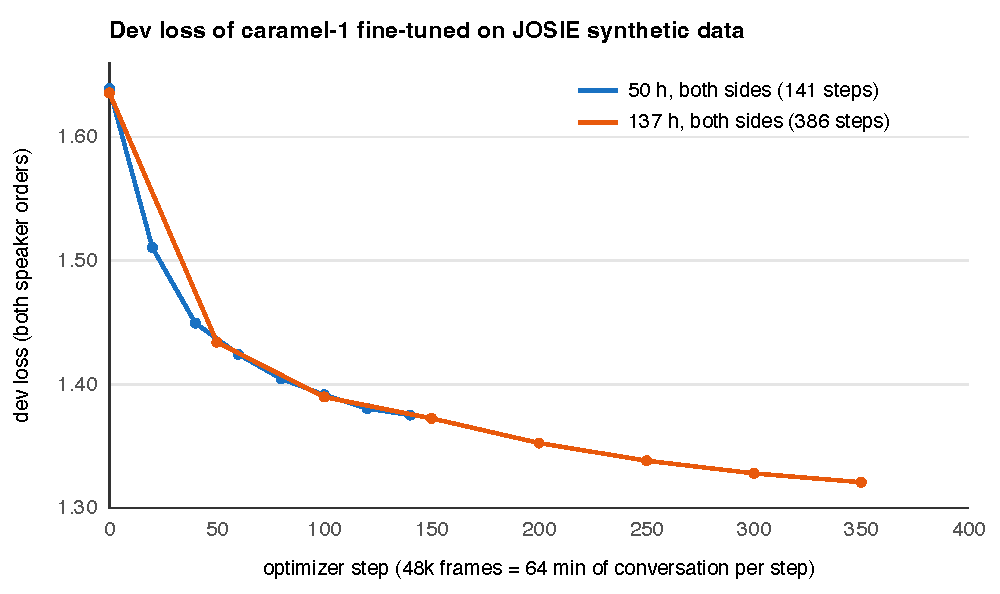
\includegraphics[width=\linewidth]{figures/plot_dev_loss.pdf}
\caption{Dev loss (swap objective).}\label{fig:dev}\end{minipage}\hfill
\begin{minipage}{.49\linewidth}\centering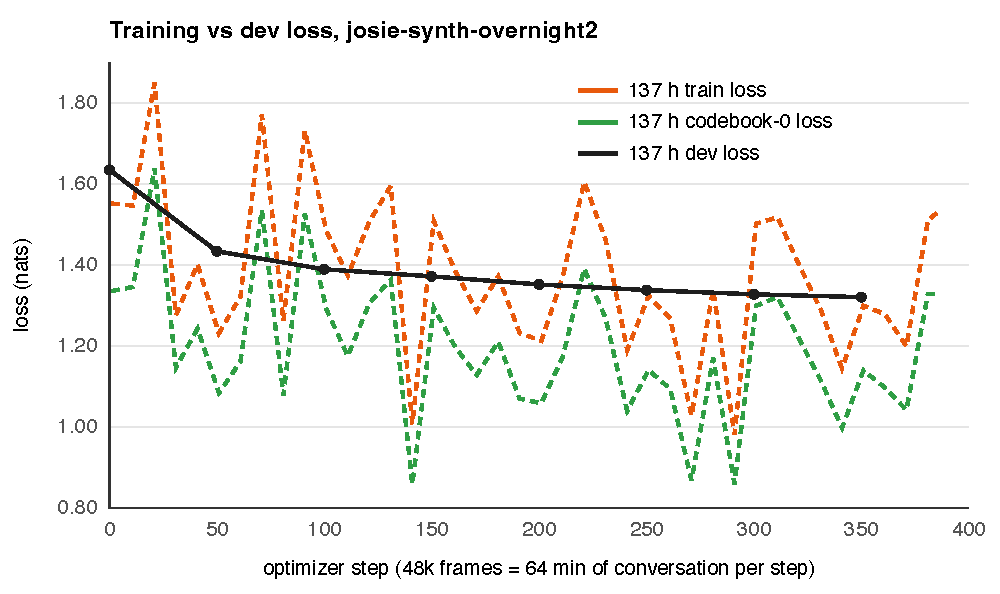
\includegraphics[width=\linewidth]{figures/plot_train_loss.pdf}
\caption{Train, codebook-0 and dev loss, 137\,h run.}\label{fig:train}\end{minipage}
\end{figure}

\paragraph{Results.} Both swap runs reduce dev loss monotonically (Fig.~\ref{fig:dev}); the 137\,h run reaches 1.321, 0.054 below the 50\,h run. Training loss is noisy because windows differ in how much speech they contain; codebook-0 loss tracks it (Fig.~\ref{fig:train}). Lower loss did not give a better assistant. In self-play from a real 12\,s opening (5 seeds, 30\,s, frame RMS $>0.01$), the \josie{} side was active 71\% of the time and the partner side 4\% (per seed 0, 0, 14, 5, 0\%), both 1\%, neither 26\%. The reference value for the partner side of \texttt{caramel-1} is about 32\%.\footnote{71/4/1/26\% are in \texttt{runs/josie-synth-overnight2/overnight.log}; the 32\% reference came from the same script in an earlier session and is not stored in the run logs.} In listening, the model talked over the user and sometimes switched into a user's (often male) voice.

\paragraph{Diagnosis.} (a) \emph{Speaker-identity leakage}: half the gradient comes from windows where the modelled stream is a user voice from 25 alternatives, so given ``I am the modelled speaker'' Zoey has weight $\frac12$ and each user voice about $\frac1{50}$. (b) \emph{Barge-in imitation}: barge-ins exist only on the user side, so Eq.~\eqref{eq:swap} rewards starting to speak over the other speaker. (c) The partner side's collapse to 4\% is consistent with the model learning that the non-assistant role is mostly silent after interruptions, together with the low prosodic diversity of synthetic speech. Eq.~\eqref{eq:aonly} removes (a) and (b) by construction (Fig.~\ref{fig:fig9_failure}).
\fig{fig9_failure}{Failure mode of the both-sides fine-tune.}

\subsection{Reinforcement learning for duplex behaviour}
\label{sec:rl}
\texttt{rl.py} implements an RL stage after the supervised fine-tune. \textbf{It has not been trained yet; no results are reported.} Each step draws $W=2$ real 60\,s windows. For each, $G=4$ rollouts are sampled: the user side is forced frame by frame from the recording (as \texttt{live.py} feeds the microphone), the first 15\,s of the assistant are real context, and afterwards the model speaks for itself (Fig.~\ref{fig:fig15_rl}). Rollouts are decoded with Mimi; frame energy above $-45$\,dBFS (with 0.4\,s gap closing and 0.16\,s minimum spurts) gives who is talking, and a 40-band log-mel profile gives whose voice it is.

\paragraph{Rewards.} Events are scored on the activity timeline from the end of the prefix on:
\begin{itemize}\itemsep0pt
\item \emph{yield}: the user barges in ($\ge$0.64\,s) while A talks: $+1$ if A falls silent within 1.0\,s and stays silent 0.32\,s, else $-1$;
\item \emph{talkover}: A starts while the user talks and overlaps for more than 1.0\,s (longer than a backchannel): $-1$;
\item \emph{respond}: the user ends a turn and A starts within 1.5\,s while the user stays quiet: $+1$;
\item \emph{dead air}: both silent for more than 3\,s, and again for every further 3\,s: $-1$;
\item \emph{voice}: per chunk of A's speech, $\cos(\mathbf{v},\mathbf{p}_A-\mathbf{c})-\cos(\mathbf{v},\mathbf{p}_U-\mathbf{c})$, with $\mathbf{v}$ the chunk's mean log-mel minus a running centre $\mathbf{c}$, $\mathbf{p}_A$ a running assistant profile and $\mathbf{p}_U$ this window's user profile.
\end{itemize}
With weights $w=(1,1,0.5,1,1)$, the reward of chunk $j$ (2\,s chunks) of rollout $i$ is $R_{ij}=\sum_e w_e\,r_{e,ij}$.

\paragraph{GRPO.} Rewards are normalised within the group of one window and turned into discounted per-chunk advantages ($\gamma=0.5$), which every token in the chunk inherits:
\begin{equation}
\hat R_{ij}=\frac{R_{ij}-\mathrm{mean}_{i'}R_{i'j}}{\mathrm{std}_{i'}R_{i'j}+10^{-4}},\qquad A_{ij}=\sum_{j'\ge j}\gamma^{\,j'-j}\hat R_{ij'}.
\end{equation}
The loss over A's sampled tokens (all 8 codebooks) is the PPO-clipped ratio plus a per-token k3 estimate of the KL to the starting model:
\begin{equation}
\mathcal{L}_\text{GRPO}=-\frac{1}{|\mathcal{T}|}\sum_{\tau\in\mathcal{T}}\Big[\min\big(\rho_\tau A_\tau,\ \mathrm{clip}(\rho_\tau,1{\pm}0.2)A_\tau\big)-\beta_\text{KL}\big(e^{\Delta_\tau}-\Delta_\tau-1\big)\Big],
\end{equation}
with $\rho_\tau=\pi_\theta/\pi_\text{old}$, $\Delta_\tau=\log\pi_\text{ref}-\log\pi_\theta$, $\beta_\text{KL}=0.02$ and learning rate $5\times10^{-7}$. An optional supervised term on the real windows can be added.
\paragraph{DPO.} Alternatively each group becomes one (best, worst) pair if their reward gap is at least 1, trained with length-normalised DPO ($\beta=0.3$):
\begin{equation}
\mathcal{L}_\text{DPO}=-\log\sigma\Big(\beta\big[\bar s(y^+)-\bar s(y^-)\big]\Big),\qquad \bar s(y)=\frac{1}{|y|}\sum_{\tau\in y}\big(\log\pi_\theta-\log\pi_\text{ref}\big).
\end{equation}
The same rewards are also computed for the real assistant track of each window, as a reference for what target behaviour scores.
\fig{fig15_rl}{The RL loop of \texttt{rl.py}.}

%=====================================================================
\section{Limitations}
\begin{itemize}\itemsep0pt
\item \textbf{Content.} \texttt{caramel-1}'s speech is human-sounding but mostly not meaningful; without a text pathway, transfer of the teacher's content through 137\,h of audio is doubtful.
\item \textbf{Detectability.} A generated-speech classifier still separates the model from real speech easily.
\item \textbf{Pending and untrained stages.} The single-side fine-tune was unfinished; synthetic stage-A pretraining and the RL stage have not been run.
\item \textbf{Evaluation of post-training.} Behavioural evidence is 5 self-play seeds, an energy-based activity measure and informal listening. We did not run the closeness score, UTMOS, ECAPA or ASR checks on the fine-tuned models.
\item \textbf{Synthetic speech.} Two TTS voice families, read prosody, no noise; a model fine-tuned only on it sounds like Phonon. About a quarter of conversations were dropped by the alignment filter, so hard-to-speak text is under-represented.
\item \textbf{Data and licences.} The pre-training corpus is scraped and not redistributable; the synthetic dataset is CC BY-NC 4.0 because the TTS is. Separation errors in the pre-training corpus were not quantified in the release.
\item \textbf{Context.} 3000 frames (240\,s) bound a conversation in the live loop.
\end{itemize}

\section{Future work}
Finish and evaluate the single-side fine-tune with the closeness score and the RL event metrics; train synthetic stage-A pretraining with random voices and real conversations mixed in (e.g.\ Seamless Interaction); run GRPO with the duplex rewards; scale pre-training data, which the release shows still lowers loss and improves clarity; and tune sampling temperature per checkpoint.

\section{Conclusion}
\caramel{} shows that a small model trained only on matched two-track conversational audio, with no text and no turn-taking rule, reproduces human conversational timing and runs in real time on a laptop. Turning it into an assistant exposes a subtle point: the speaker-swap augmentation that makes self-play possible is the wrong objective for asymmetric assistant data, because it teaches the model to be the user. A single-side objective after symmetric pretraining, followed by RL on duplex events, is the principled route; its evaluation is the next step.

\bibliographystyle{plainnat}
\bibliography{references}

\appendix
\section{Hyperparameters}
{\small\begin{longtable}{lp{6.2cm}p{5.4cm}}\toprule
group & parameter & value\\\midrule
\endhead
codec & sample rate / frame / codebooks / vocabulary & 24 kHz / 1920 samples (80 ms) / 8 / 2048\\
model & $n_q$, $K$ (dep\_q), delays & 16, 8, $(0,1^7,0,1^7)$\\
temporal & $d$, layers, heads, $d_\text{ff}$, RoPE base, context & 1024, 16, 16, 2816, $10^4$, 3000 frames\\
depformer & $d'$, layers, heads, $d'_\text{ff}$ & 512, 6, 8, 1408\\
model & parameters & 413{,}198{,}848\\
optimiser & AdamW $\beta$, $\epsilon$, weight decay, clip & (0.9, 0.95), $10^{-8}$, 0.1 (matrices), 1.0\\
schedule & warm-up, floor & 50 steps default (stage 3: 200), $0.1\eta_{\max}$\\
pre-training & $\eta_{\max}$ stages 1--2 / 3 & $3\times10^{-4}$ / $1.5\times10^{-4}$\\
batching & frames per step, micro-batch, accumulation & 48{,}000, 6{,}000, 8\\
batching & window buckets & 750, 1000, 1250, 1500 frames\\
batching & store weights (stage 2--3) & 0.8 stereo, 0.2 mono\\
eval & dev windows, length & 64 $\times$ 1{,}500 frames, both orders\\
sampling & temperature, top-$k$ & 1.1, 50\\
\josie{} SFT & $\eta_{\max}$, epochs, steps, objective & $10^{-4}$, 3, 386, swap / \texttt{--no\_swap}\\
data & barge-in, wait, listen, backchannel, check-in & 0.25, 0.10, 0.10, 0.2, 0.5\\
data & assistant stop after barge-in, max hold, align threshold & 750 ms, 60 s, 0.8\\
RL & windows, group, window, prefix & 2, 4, 60 s, 15 s\\
RL & lr, warm-up, clip $\epsilon$, KL, $\gamma$, chunk & $5\times10^{-7}$, 10, 0.2, 0.02, 0.5, 2 s\\
RL & rollout temperature, top-$k$, DPO $\beta$, margin & 1.0, 250, 0.3, 1.0\\
RL & reward weights (yield, talkover, respond, dead air, voice) & 1, 1, 0.5, 1, 1\\
RL & VAD threshold, gap, min spurt & $-45$ dBFS, 0.4 s, 0.16 s\\\bottomrule
\end{longtable}}

\section{Reproducibility}
\begin{itemize}\itemsep0pt
\item \textbf{Weights}: \url{https://huggingface.co/naklecha/caramel-1}; \texttt{setup.sh} installs MLX and \texttt{mlx-audio} and downloads them.
\item \textbf{Data}: \texttt{prepare.py} builds token stores (Seamless Interaction with \texttt{--pair\_regex}, otoSpeech with \texttt{--stereo}, Libri-Light \texttt{medium} as mono).
\item \textbf{Pre-training}: \texttt{train.py} stage 1 (\texttt{--steps 25000 --stop\_at 9000}), stage 2 (\texttt{--resume}, weights 0.8/0.2), stage 3 (\texttt{--sched\_start 25000 --warmup 200 --lr 1.5e-4 --save\_best}), as in the README.
\item \textbf{Inference}: \path{generate.py} (self-play, \path{--prompt}, \path{--bits}, \path{--realtime}) and \texttt{live.py} (microphone or \texttt{--mic\_file}).
\item \textbf{Post-training}: \texttt{synthetic\_data.ipynb} and \texttt{synthetic\_pretrain.ipynb} generate data; \texttt{train.py --data hf://Goekdeniz-Guelmez/josie-live-synthetic --no\_swap}; \texttt{rl.py --algo grpo|dpo}.
\item \textbf{This report}: \path{paper/scripts/figures.py} and \path{paper/scripts/figures2.py} build the figures (Excalidraw sources in \path{paper/figures/}); \path{paper/scripts/plots.py} builds the plots from \path{runs/*/train.log}.
\end{itemize}
\end{document}
